\chapter{Architectural Views} \label{ArchitecturalViews}


\section{Context View}

\subsection{Stakeholders’ uses of this view}
The key use of the Context View for the stakeholders of \cite{farmbot} FarmBot is to ensure that the overall end-to-end solution indeed sensibly satisfies functionality requirements from a general viewpoint. The different stakeholders' uses of this view are as follows:
\begin{itemize}
    \item Developers: Use the context view in order to have a better picture of how the system fits into the overall application landscape. They use it to understand the interactions with external systems and entities. In addition to that, for further improvements to the system, they can better assess completeness, consistency and coherence.
    \item End Users (Students, Researchers, Home Users, Artwork Creators): Use the context view in order to ensure that FarmBot is able to satisfy their requirements and its' scope is correct. Also it enables them to learn how the data flows, the interactions are done throughout the FarmBot system and what external entities or services are part of it.
    \item Ministry of Agriculture: Use the context view for auditing FarmBot as a system, see what external entities and services are used, where and how data flows.
\end{itemize}

\subsection{Context Diagram}

% Context Diagram should display all external entities that may interact with the system. This section should include a \textbf{Context Diagram and explanations} for the context diagram.

The FarmBot is a standalone system that interacts with four external entities as shown in Figure \ref{fig:ContextDiagram}:

\begin{figure}[H]
    \centering
    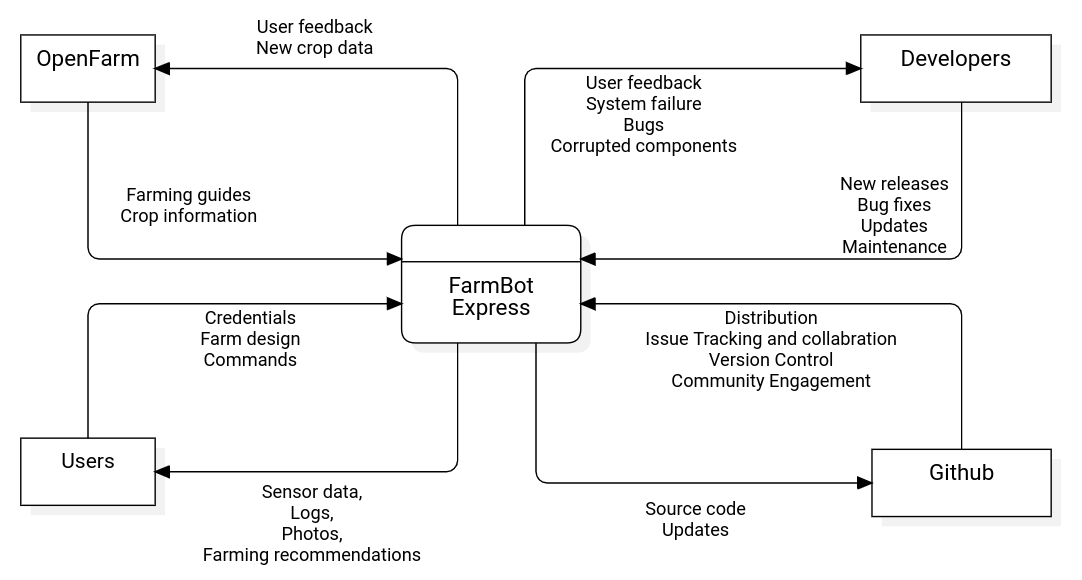
\includegraphics[width=1\textwidth]{Figures/ContextDiagram.png}
    \caption{FarmBot Context Diagram}\label{fig:ContextDiagram}
\end{figure}

\begin{itemize}
    \item \textbf{Users:} The user interacts with the system through the web application. The user can create, edit, and delete sequences, view the status of the FarmBot, and monitor the progress of the FarmBot. The user provides data to the system, such as the location of the FarmBot, the type of plants, and the planting schedule. The user can also receive data from the system such as the status of the FarmBot and the progress of the FarmBot.
    \item \textbf{Developers:} The developers are responsible for maintaining the system and ensuring that it is operational. They can access the system through the web application and perform maintenance tasks. Furthermore, they can update the system and add new features.
    \item \textbf{OpenFarm:} The OpenFarm is an open-source database system that contains information about plants and crops. It can be considered a data store (a shared database) external to the system. The system interacts with OpenFarm to retrieve information about plants and crops. This information is used to determine the planting schedule and the requirements of the plants.
    \item \textbf{GitHub:} The \gls{github} is a version control system that stores the system's source code. The system interacts with GitHub to retrieve the source code and update the system. The developers can access the source code through GitHub and make changes to the system. In addition, it encourages community engagement and collaboration.
\end{itemize}

\subsection{External Interfaces}
% This section should include an \textbf{External Interfaces Class Diagram}. Descriptions of the operations given in the external interface class diagram should also be given. \textbf{You should aim for 3 external interfaces.}

The FarmBot interacts with four external entities as shown in Figure \ref{fig:ExternalInterfacesClassDiagram}:
\begin{figure}[H]
    \centering
    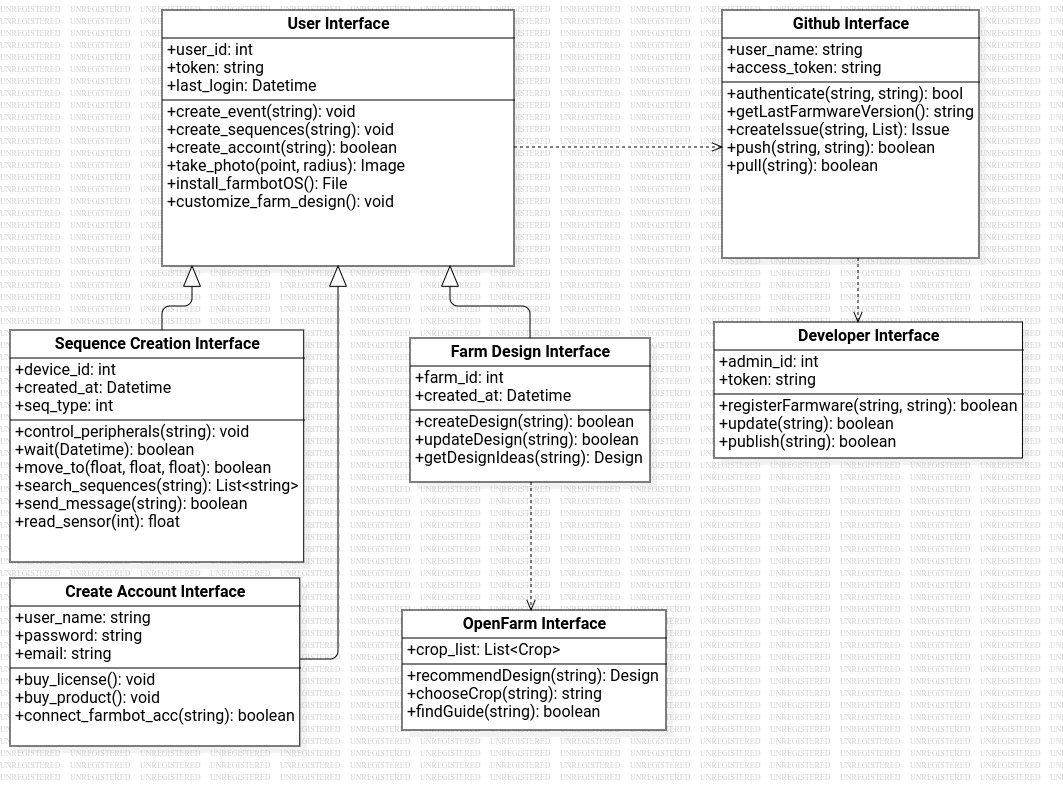
\includegraphics[width=155mm]{Figures/ClassDiagram.jpg}
    \caption{FarmBot External Interfaces Class Diagram}\label{fig:ExternalInterfacesClassDiagram}
\end{figure}

\begin{itemize}
    \item \textbf{User Interface:} The User Interface is responsible for handling the user interactions with the system. It provides the user with a graphical user interface (GUI) that allows the user to interact with the system. The User Interface receives input from the user and sends it to the system. It also receives output from the system and displays it to the user. The User Interface is implemented as a web application that can be accessed through a web browser. It can be considered as an event provider or consumer in our case.
    \item \textbf{Developer Interface:} The developer interface is used to interact with the system for development purposes. Developers can create new features, fix bugs, etc. Developers use this interface to contribute to the system. With further investigation, one can see that users depend on this interface to get the latest version of the software since the maintenance of the GitHub interface depends on developers.
    \item \textbf{OpenFarm Interface:} The OpenFarm Interface is responsible for interacting with the OpenFarm database. It retrieves information about plants and crops from the OpenFarm database. The OpenFarm Interface sends requests to the OpenFarm database and receives responses from the OpenFarm database. The OpenFarm Interface is implemented as a RESTful API that can be accessed over the internet. It can be considered as a data or service provider in our case.
    \item \textbf{GitHub Interface:} The GitHub Interface is responsible for interacting with the GitHub version control system. It retrieves the source code of the system from the GitHub repository. The GitHub Interface sends requests to the GitHub repository and receives responses from the GitHub repository. Furthermore, it provides users and developers with a forum to collaborate and contribute to the system. The GitHub Interface is implemented as a web application that can be accessed through a web browser. It can be considered as a data or service provider in our case.
\end{itemize}

\subsection{Interaction scenarios}
% This section includes \textbf{2 Activity Diagrams} to show interaction sequences taking place over the external interfaces. Choose the 2 most complex interactions for activity diagrams. They must be different from those in your \gls{srs} document.


\begin{figure}[H]
    \centering
    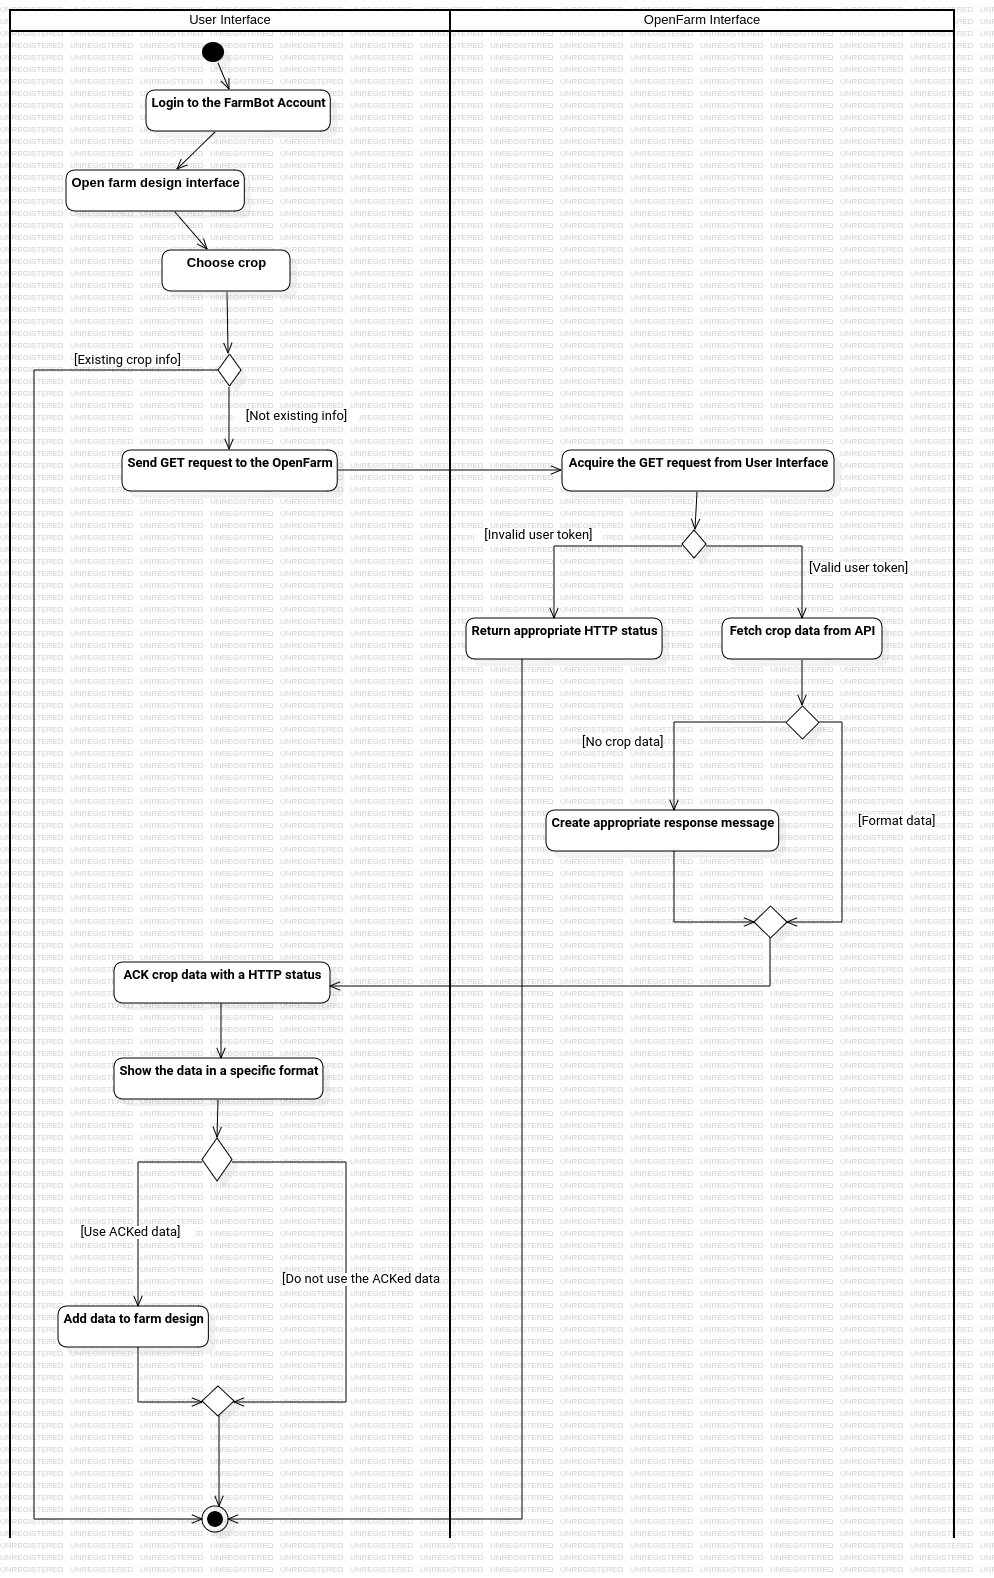
\includegraphics[width=0.95\textwidth]{Figures/ActivityDiagram_openfarmPipeline.png}
    \caption{Activity diagram between User Interface and OpenFarm Interface}\label{fig:ActivityDiagram_openfarmPipeline}
\end{figure}

The activity diagram in Figure~\ref{fig:ActivityDiagram_openfarmPipeline} shows the interaction between the User Interface and the OpenFarm Interface. The User Interface sends a request to the OpenFarm Interface to retrieve information about plants and crops. The User Interface can request the OpenFarm Interface to retrieve information about a specific plant or crop. The OpenFarm Interface responds to the User Interface with information about the specific plant or crop. The User Interface displays the information to the user.


\begin{figure}[H]
    \centering
    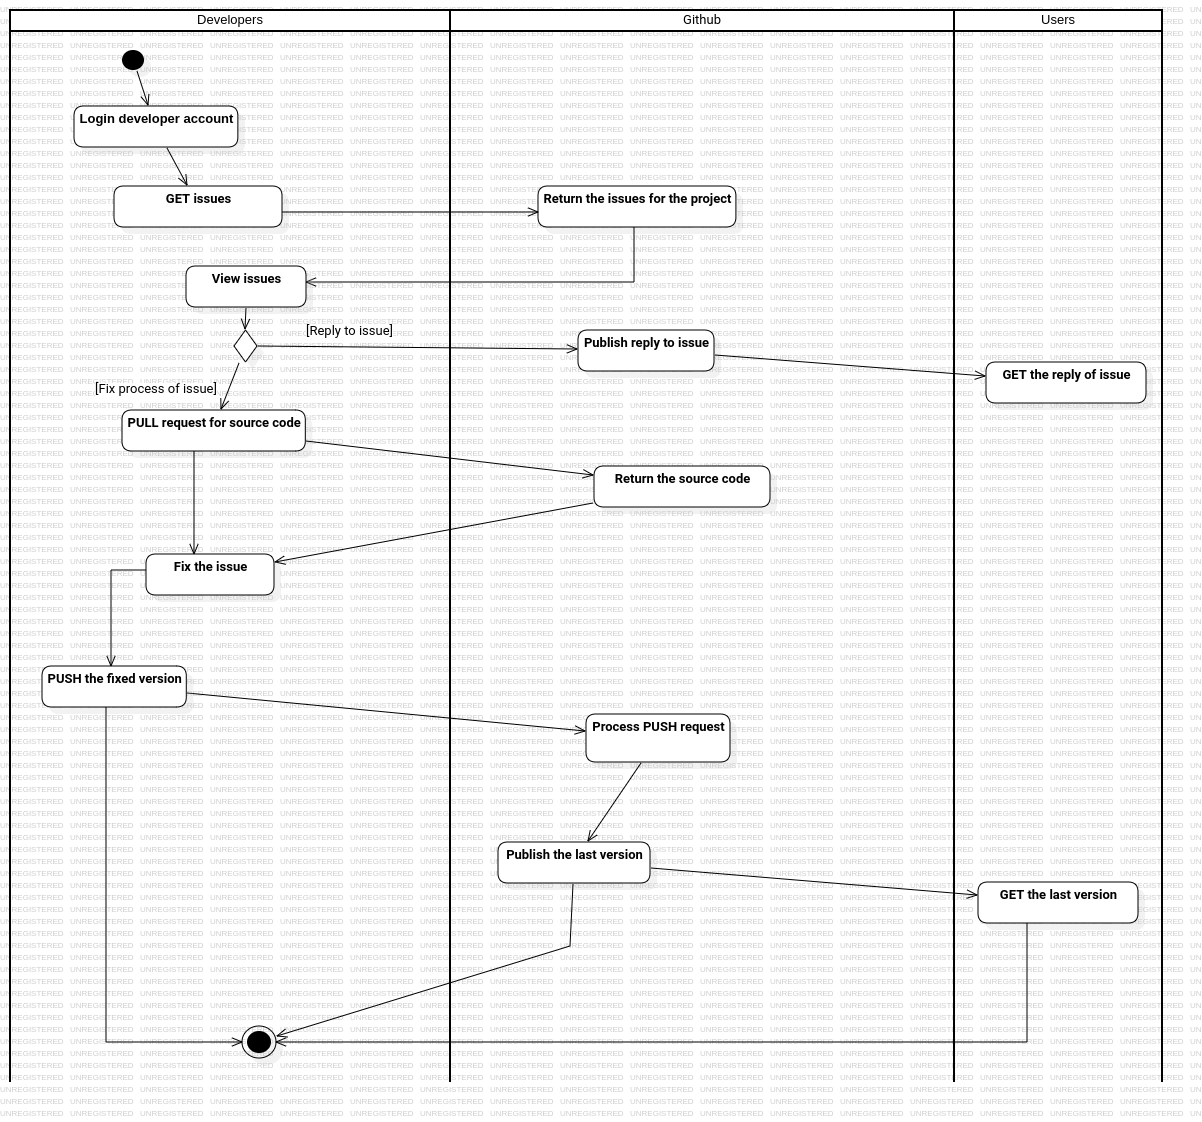
\includegraphics[width=1\textwidth]{Figures/ActivityDiagram_maintanencepipeline.png}
    \caption{Activity diagram of a Maintenance Pipeline}\label{fig:ActivityDiagram_maintanencepipeline}
\end{figure}

The activity diagram in Figure~\ref{fig:ActivityDiagram_maintanencepipeline} shows the interaction between the Developer, \gls{github}, and the user interface; it shows a basic instance of a maintenance action. The developer sends a request to the \gls{github} Interface to retrieve the system's source code. The \gls{github} Interface responds to the Developer with the system's source code. The Developer changes the source code and sends a request to the \gls{github} Interface to update the system. The \gls{github} Interface updates the system with the changes made by the Developer. The User Interface displays the updated system to the user.



\section{Functional View} 

\subsection{Stakeholders’ uses of this view}
The Functional View offers an overview of how architectural elements work together to provide the various functionalities of FarmBot. Below, you can find the FarmBot Stakeholders' uses of this view:
\begin{itemize}
    \item \textbf{Developers}: The developers' main concern is the quality of design and the internal structure of the FarmBot system. The internal structure is crucial to meet the desired quality requirements such as availability, ability to scale, security during development. Also developers can use this view to see the external interfaces.
    \item \textbf{End Users} (Students, Researchers, Home Users, Artwork Creators): End users can use this view to learn the functionalities provided by FarmBot and how they are provided, what external interfaces are used.
    \item \textbf{Ministry of Agriculture}: Their use of this view is to have a more in-depth knowledge of the overall system, internal structure, external interfaces, and functionality for auditing.
\end{itemize}

\subsection{Component Diagram}

\begin{figure}[H]
    \centering
    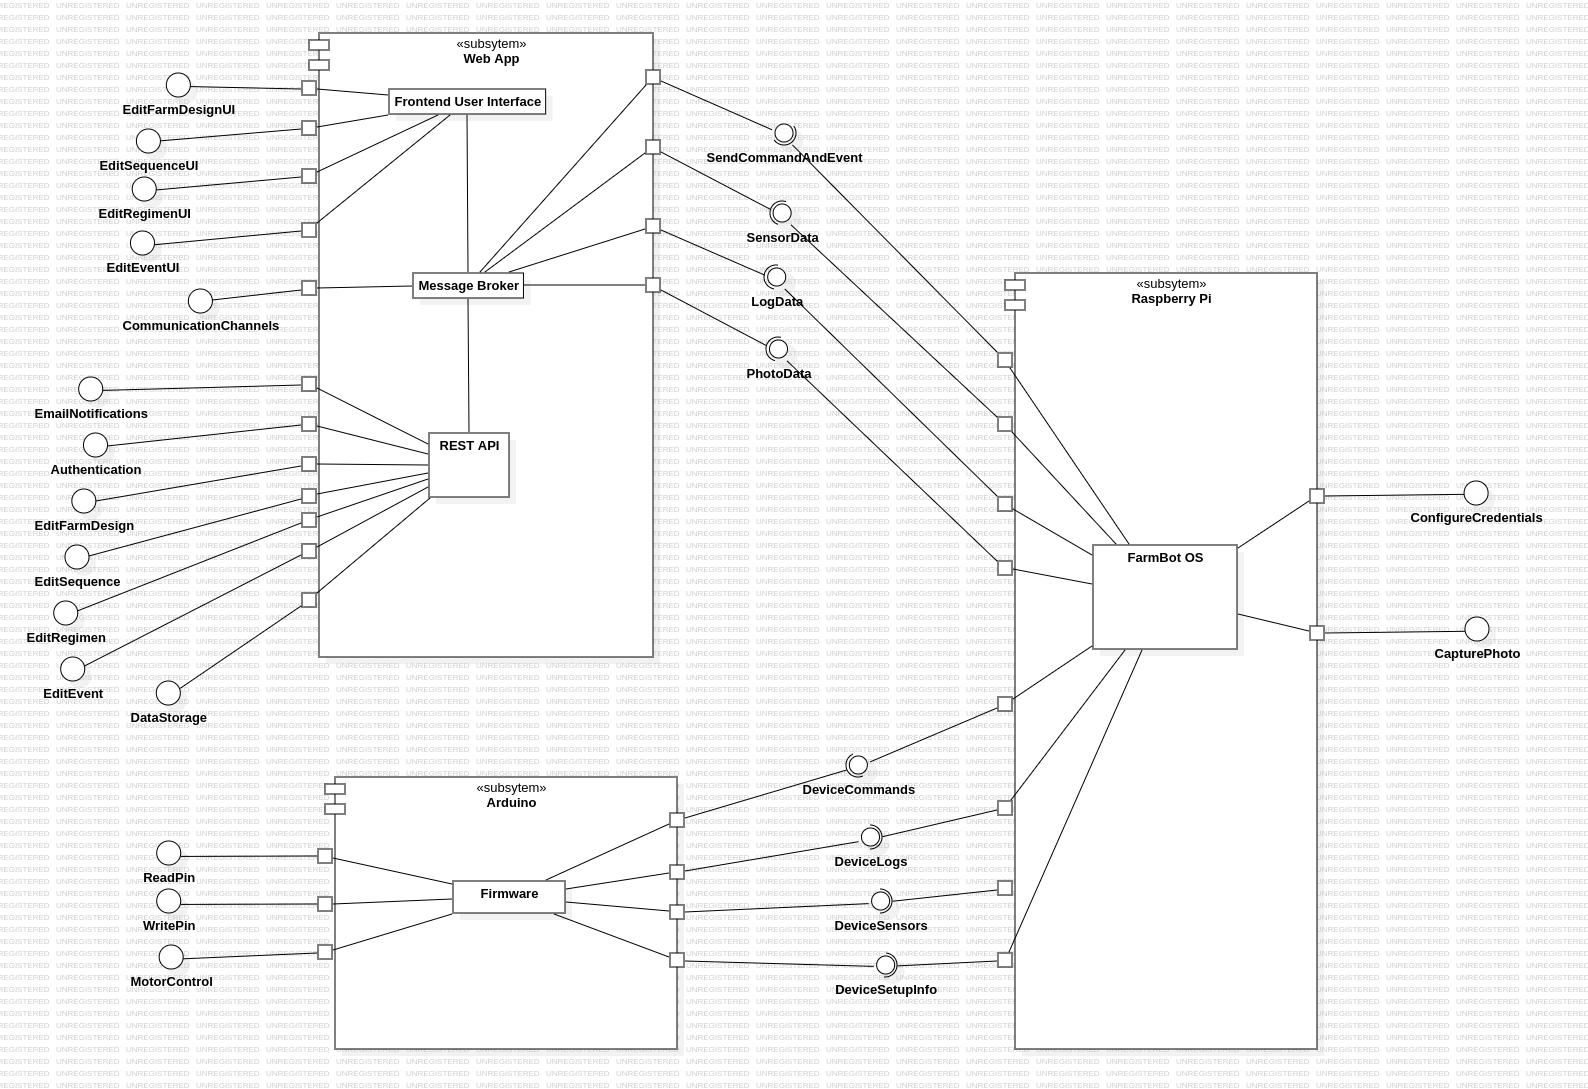
\includegraphics[width=0.95\textwidth]{Figures/ComponentDiagram.png}
    \caption{Component Diagram for FarmBot}\label{fig:ComponentDiagram}
\end{figure}

The Component Diagram for FarmBot consists of three subsystems: Web App, Raspberry Pi, and Arduino.
\begin{itemize}
    \item \textbf{Web App:} The Web App has three parts in Frontend User Interface, Message Broker, and REST API. 
    \begin{itemize}
        \item \textbf{The Frontend User Interface} provides UI elements for the end user to design their farm, edit, and create sequences, regimens, or events.
        \item \textbf{The Message Broker} provides communication between FarmBot device and WebApp. The device is controlled through the message broker. It handles photo, sensor and log data flow. The commands, events of user are sent through it. Provides an external interface for different communcation channels.
        \item \textbf{The REST API} provides the functionality for user actions with the Web App such as editing farm design, sequences, regimens, and events. It provides long term data storage and authentication. 
    \end{itemize}
    \item \textbf{Raspberry Pi:} The Raspberry Pi componenet consists of FarmBot OS. FarmBot OS provides external interfaces for device configuration (WIFI and account credentials) and capturing photos. In addition, it provides interfaces to the message broker for the flow of photo, log, and sensor data. It generates G and F code commands from high level user commands then passes them to the FarmBot device.
    \item \textbf{Arduino:} The Arduino consists of the firmware. It provides external interfaces for reading and writing device pins, and controlling the motors. In addition, it executes commands that were passed by FarmBot OS and provides device logs, sensor data and setup information of pins and encoders back.
    
\end{itemize}

\subsection{Internal Interfaces}

\begin{figure}[H]
    \centering
    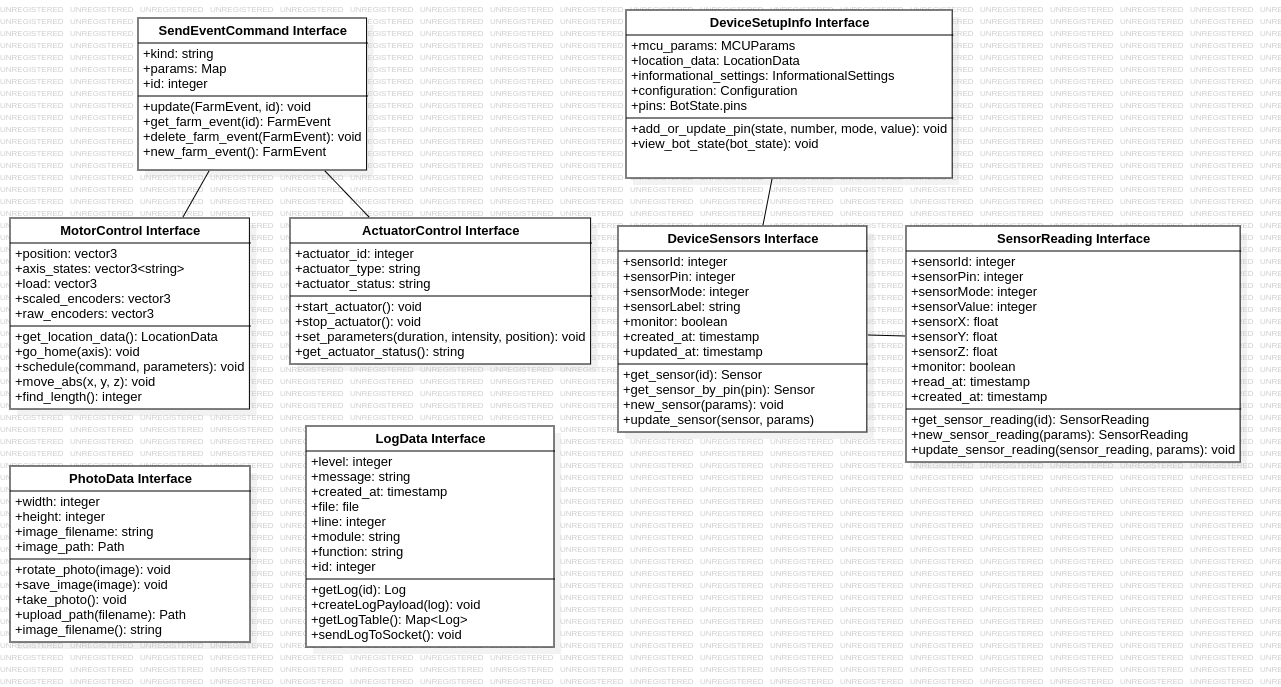
\includegraphics[width=1\textwidth]{Figures/Internal_Interface_Diagram.png}
    \caption{FarmBot Internal Interface Diagram}\label{fig:InternalInterfaceDiagram}
\end{figure}

\begin{itemize}
    \item \textbf{PhotoData Interface:} \begin{itemize}
        \item \textbf{width}: The width of the image
        \item \textbf{height}: The height of the image
        \item \textbf{image\_filename}: The stored filename of the image with timestamp
        \item \textbf{image\_path}: The path of the stored image used for uploading the image
        \item \textbf{rotate\_photo(image)}: Rotates the captured if the calibration data exists.
        \item \textbf{save\_image(image)}: Saves the captured image to a file after modifying operations
        \item \textbf{take\_photo()}: Takes a photo using the connected camera
        \item \textbf{upload\_path(filename)}: Returns the path for the image file to be uploaded.
        \item \textbf{image\_filename()}: Prepares and returns the filename with timestamp.
    \end{itemize}
    
    \item \textbf{SendCommandAndEvent Interface:} \begin{itemize}
        \item \textbf{kind}: The type of the command asset (FarmEvent, Regimen etc.)
        \item \textbf{params}: A key value map of changes to be made with the command.
        \item \textbf{id}: The id of the remote database that stores events and commands.
        \item \textbf{update(FarmEvent, id)}: Updates the FarmEvent stored in the database.
        \item \textbf{get\_farm\_event(id)}: Returns the FarmEvent with the given id.
        \item \textbf{delete\_farm\_event(id)}: Deletes the FarmEvent with the given id from the database.
        \item \textbf{new\_farm\_event()}: Creates and returns a new FarmEvent.
    \end{itemize}
    
    \item \textbf{MotorControl Interface:} \begin{itemize}
        \item \textbf{position}: A vector with three components storing the position of the FarmBot
        \item \textbf{axis\_states}: A vector with three components storing the position of the FarmBot with string representation
        \item \textbf{load}: A vector with three componenets that stores the load on each axis of the FarmBot
        \item \textbf{scaled\_encoders}: A vector with three components that hold the rotation of each motor axis, scaled with the correct motor\_resolution.
        \item \textbf{raw\_encoders}: A vector with three components that hold the raw rotation values of each motor axis.
        \item \textbf{get\_location\_data()}: Returns the location data of the FarmBot device.
        \item \textbf{go\_home(axis)}: Commands the FarmBot device to move to its home position regarding to the given axis.
        \item \textbf{move\_abs(x, y, z)}: Move to the given location with absolute coordinates.
        \item \textbf{schedule(command, parameters)}: Communicates with the Arduino \newline firmware in G Code to start executing the command.
        \item \textbf{find\_length(axis)}: Find the length of the given axis.
    \end{itemize}

    \item \textbf{ActuatorControl Interface:} \begin{itemize}
        \item \textbf{actuator\_id}: The ID of the actuator
        \item \textbf{actuator\_type}: An indicator of the type of actuator (e.g., watering pump, linear actuator, LED light strip).
        \item \textbf{actuator\_status}: Indicates the current state of the actuator (e.g., on, off, idle, busy).
        \item \textbf{start\_actuator()}: Starts the actuator
        \item \textbf{stop\_actuator()}: Stops the actuator
        \item \textbf{set\_parameters(duration, intensity, position)}: Sets the parameters of actuator for executing its action
        \item \textbf{get\_actuator\_status()}: Returns the current state of the actuator
    \end{itemize}

    \item \textbf{SensorReading Interface:} \begin{itemize}
        \item \textbf{sensorId}: The ID of the sensor.
        \item \textbf{sensorPin}: The pin of the sensor on the FarmBot device.
        \item \textbf{sensorMode}: The I/O mode of the sensor.
        \item \textbf{sensorValue}: The value of the sensor.
        \item \textbf{sensorX}: The X position of the sensor.
        \item \textbf{sensorY}: The Y position of the sensor.
        \item \textbf{sensorZ}: The Z position of the sensor.
        \item \textbf{monitor}: A boolean value set if the sensor will be monitored.
        \item \textbf{read\_at}: The timestamp of last reading from sensor.
        \item \textbf{created\_at}: The timestamp when the sensor was first created.
        \item \textbf{get\_sensor\_reading(id)}: Returns the latest reading from the sensor with the given id.
        \item \textbf{new\_sensor\_reading(params)}: Creates a new sensor reading from the sensor using the params.
        \item \textbf{update\_sensor\_reading(sensor\_reading, params)}: Updates an existing sensor\_reading using the given params.
    \end{itemize}

    \item \textbf{DeviceSensors Interface:} \begin{itemize}
        \item \textbf{sensorId}: The ID of the sensor.
        \item \textbf{sensorPin}: The pin of the sensor
        \item \textbf{sensorMode}: The I/O mode of the sensor
        \item \textbf{sensorLabel}: The string label attached to the sensor.
        \item \textbf{monitor}: A boolean value set if the sensor will be monitored.
        \item \textbf{created\_at}: The creation timestamp of sensor.
        \item \textbf{updated\_at}: The update timestamp of sensor.
        \item \textbf{get\_sensor(id)}: Returns the sensor with the given id.
        \item \textbf{get\_sensor\_by\_pin(pin)}: Returns the sensor that is connected to the given pin.
        \item \textbf{new\_sensor(params)}: Creates a new sensor using the given parameters.
        \item \textbf{update\_sensor(sensor, params)}: Updates the given sensor with the given parameters.
    \end{itemize}
    
    \item \textbf{DeviceSetupInfo Interface:} \begin{itemize}
        \item \textbf{mcu\_params}: Holds hardware parameter information regarding the device such as encoders, pins, movement settings of motors.
        \item \textbf{location\_data}: Holds the current location data of the device.
        \item \textbf{informational\_settings}: Holds general information about the hardware device status such as firmware version, controller version, WiFi level, up-time, memory usage.
        \item \textbf{configuration}: Holds the configuration settings of firmware such as firmware hardware, input-output logs, debug logs, auto-update settings.
        \item \textbf{pins}: Holds the pin information for the device.
        \item \textbf{add\_or\_update\_pin(state, number, mode, value)}: Updates the value of a given pin with number, state and mode. In the case it does not already exist, adds new pin.
        \item \textbf{view\_bot\_state(bot\_state)}: Returns a view of the current state of the FarmBot such as position, pins, stall status.
    \end{itemize}

    \item \textbf{LogData Interface:}
    \begin{itemize}
        \item \textbf{level}: The level of the log indicating the type such as debug, info, error, warn, success.
        \item \textbf{message}: The message string to be logged.
        \item \textbf{created\_at}: The timestamp of the log creation.
        \item \textbf{file}: The file associated with the log entry.
        \item \textbf{line}: The line of file associated with the log entry.
        \item \textbf{module}: The software module associated with the log entry.
        \item \textbf{function}: The function that is associated with the log entry.
        \item \textbf{id}: The id of the log.
        \item \textbf{get\_log(id)}: Returns the log with the given id.
        \item \textbf{create\_log\_payload(log)}: Creates a log payload to be sent over the network.
        \item \textbf{get\_log\_table()}: Returns a map of id and logs for all logs.
        \item \textbf{send\_log\_to\_socket()}: Sends the created log payload over the network to the web socket.
    \end{itemize}

    
\end{itemize}

%This section should include an \textbf{Internal Interfaces Class Diagram}. Descriptions of the operations given in the internal interface class diagram should also be given. \textbf{You should aim for 4 internal interfaces.}

\subsection{Interaction Patterns}
\begin{figure}[H]
    \centering
    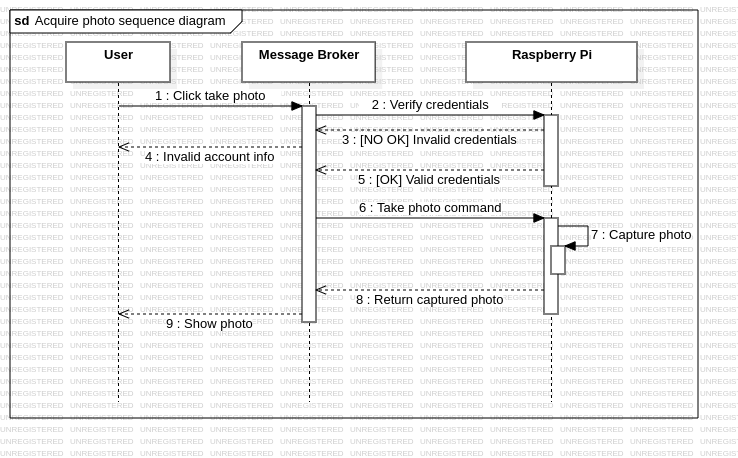
\includegraphics[width=1\textwidth]{Figures/SequenceDiagarm_photo.png}
    \caption{Acquire Photo Sequence Diagram}\label{fig:SequenceDiagram1}
\end{figure}


The sequence diagram in Figure~\ref{fig:SequenceDiagram1} shows the interaction between the \textbf{User}, \textbf{Message Broker} (FarmBot Web App) and \textbf{Raspberry Pi}. The \textbf{User} sends a request to the \textbf{Message Broker} to acquire a photo. The \textbf{Message Broker} sends a request to the \textbf{Raspberry Pi} to acquire a photo. The \textbf{Raspberry Pi} acquires the photo and sends it to the \textbf{Message Broker}. The \textbf{Message Broker} sends the photo to the \textbf{User}.

\begin{figure}[H]
    \centering
    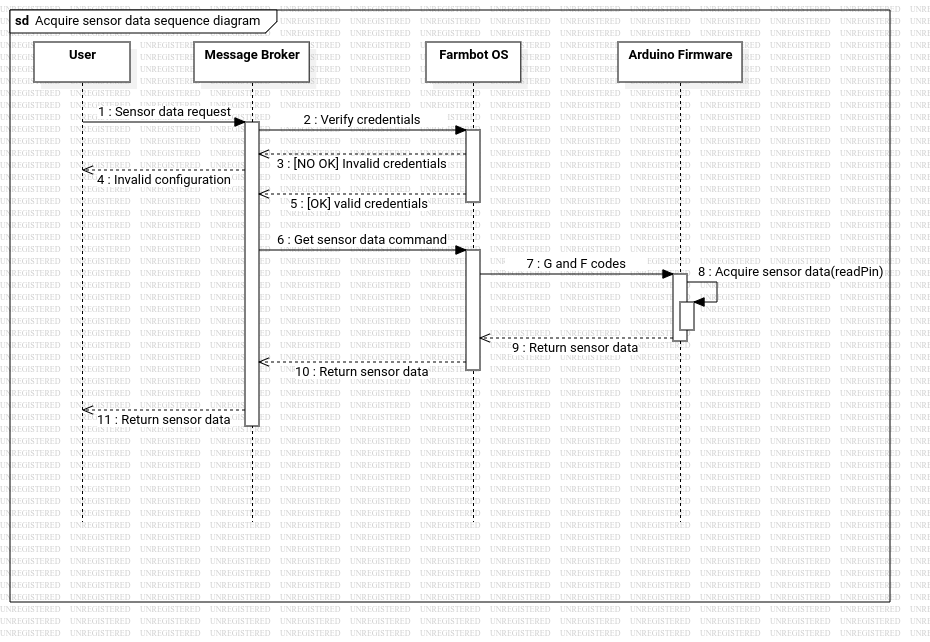
\includegraphics[width=1\textwidth]{Figures/SequenceDiagarm_sensorData.png}
    \caption{Acquire Sensor Data Sequence Diagram}\label{fig:SequenceDiagram2}
\end{figure}

The sequence diagram in Figure~\ref{fig:SequenceDiagram2} shows the interaction between the \textbf{User}, \textbf{Message Broker} (FarmBot Web App) and \textbf{FarmBot OS} (Raspberry Pi), and the \textbf{Arduino Firmware}. The \textbf{User} sends a request to the \textbf{Message Broker} to acquire sensor data. The \textbf{Message Broker} sends a converted command to the Raspberry Pi's OS to acquire sensor data. The OS creates related G and F codes that can be encoded/decoded in the \textbf{Arduino Firmware}. The \textbf{Arduino Firmware} acquires the sensor data and sends it to the \textbf{User}.

\begin{figure}[H]
    \centering
    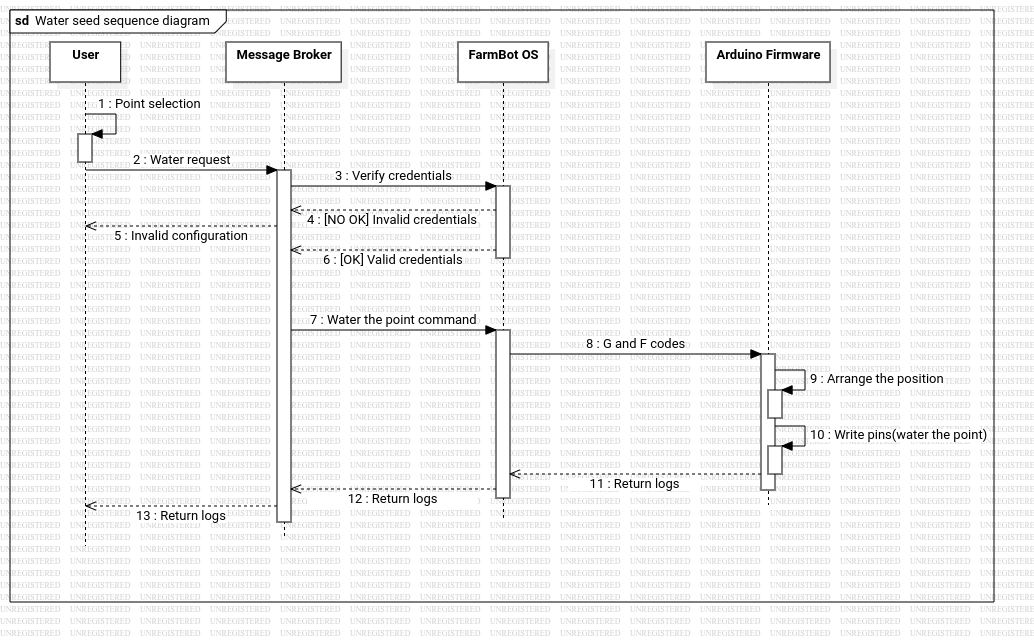
\includegraphics[width=1\textwidth]{Figures/SequenceDiagram_watering.png}
    \caption{Watering Crop Sequence Diagram}\label{fig:SequenceDiagram3}
\end{figure}

The sequence diagram in Figure~\ref{fig:SequenceDiagram3} shows the interaction between the \textbf{User}, \textbf{Message Broker} (FarmBot Web App), \textbf{FarmBot OS} (Raspberry Pi), and the \textbf{Arduino Firmware}. The \textbf{User} sends a request to the \textbf{Message Broker} to water the crops at the specified coordinates (point). The \textbf{Message Broker} sends a converted command to the Raspberry Pi's OS to water the crops at the specified coordinates. The OS creates related G and F codes that can be encoded/decoded in the \textbf{Arduino Firmware}. The \textbf{Arduino Firmware} waters the crops at the specified coordinates and sends the status (logs) to the \textbf{User}.


\section{Information View}

% Refer to \textit{R\&W Chapter 18}.

\subsection{Stakeholders’ uses of this view}

The key use of the \textbf{Information View} for the stakeholders of FarmBot is to ensure that the data requirements are correctly understood and that the data is stored and handled correctly. The different stakeholders' uses of this view are as follows:
\begin{itemize}
    \item \textbf{End users:} The end users primarily interact with the information view to understand the data being collected by FarmBot and how it relates to their gardening activities. They may use this view to monitor plant health, track growth progress, and receive alerts or recommendations.
    \item \textbf{Developers:} Developers use the information view to design and implement features related to data collection, storage, and processing. They ensure that the data is collected efficiently, stored securely, and can be accessed and manipulated as needed for various functionalities.
    \item \textbf{Ministry of Agriculture:} The Ministry of Agriculture utilizes the information view to oversee and regulate the use of FarmBot data for agricultural purposes. They may use this view to monitor farming practices, analyze trends, and make informed decisions regarding agricultural policies and practices.
    \end{itemize}
\subsection{Database Class Diagram}

% \textbf{Database Class Diagram} involving the key database or main memory objects. Complete with relevant associations. Descriptions of the non-obvious names (for classes, attributes, operations) should also be given.
\begin{figure}[H]
    \centering
    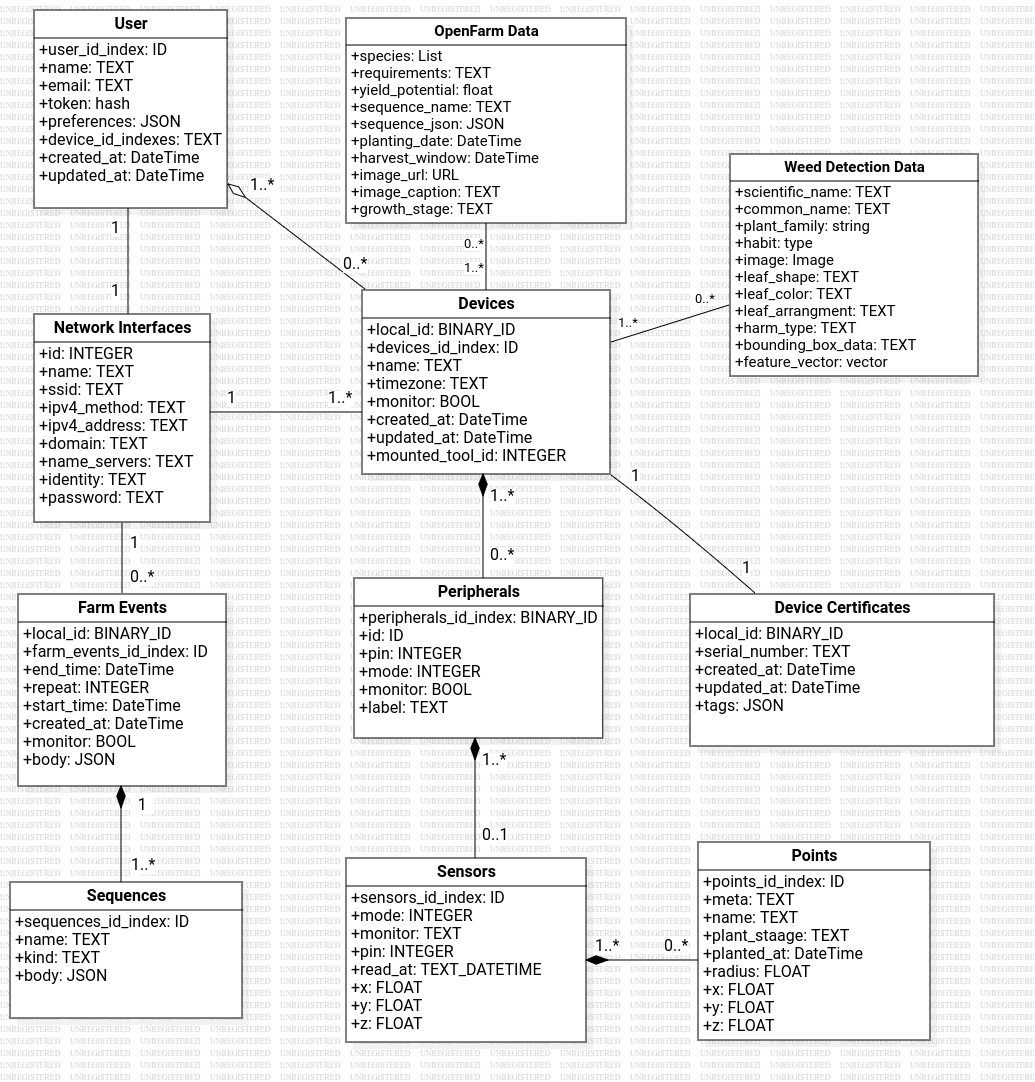
\includegraphics[width=1\textwidth]{Figures/DBDiagram.png}
    \caption{FarmBot Database Class Diagram}\label{fig:DatabaseClassDiagram}
\end{figure}

The \textbf{Database Class Diagram} in Figure~\ref{fig:DatabaseClassDiagram} shows the key database objects used by the FarmBot system. The database objects include \textbf{user, device, network interface, farm events, sequences, etc.}. Some of the main tables explained in the diagram are as follows:
\begin{itemize}
    \item \textbf{User:} The \textbf{user} object represents the user of the system. It contains information about the user, such as the user's name, email address, and password.
    \item \textbf{Device:} The \textbf{device} object represents the FarmBot device. It contains information about the device, such as its name, location, and status.
    \item \textbf{Network Interface:} The \textbf{network interface} object represents the network interface of the FarmBot device. It contains information about the network interface, such as the network interface's name, IP address, and status.
    \item \textbf{Farm Events:} The \textbf{farm events} object represents the events that occur on the farm. It contains information about the farm events, such as the event's name, date, and description.
    \item \textbf{Sequences:} The \textbf{sequences} object represents the sequences of actions that the FarmBot device can perform. It contains information about the sequences, such as the sequence's name, description, and actions.
    \item \textbf{OpenFarm Data:} The \textbf{open farm data} object represents the data retrieved from the OpenFarm database. It contains information about the plants and crops, such as the plant's name, description, and requirements.
    \item \textbf{Sensors:} The \textbf{sensors} object represents the sensors on the FarmBot device. It contains information about the sensors, such as their name, type, and status.
    \item \textbf{Points:} The \textbf{points} object represents the points on the farm. It contains information about the points, such as their name, location, and status.
    \item \textbf{Weed Detection Data:} The \textbf{weed detection data} object represents the data collected by the weed detection system. It contains information about the weed detection data, such as the data's name, location, and status. It can be used to detect and remove weeds from the farm. The data stored in this table can be used in image processing algorithms to detect and remove weeds from the farm. Furthermore, using bounding box data and feature vectors of the detected weeds, some AI algorithms can be used to classify and remove the weeds.
\end{itemize}
\subsection{Operations on Data}
% Descriptions of the operations are given in the database class diagram. These operations may deal with the storage and handling of information regarding stores, customers, products, and so on. \textbf{Operations should be listed in a table or using bullets.}
% These usually include CRUD (Create Read Update Delete) operations.

\begin{longtable}[c]{|l|l|}
    \hline
    Operation        & Description                                                                                             \\ \hline
    \endfirsthead
    %
    \multicolumn{2}{c}%
    {{\bfseries Table \thetable\ continued from previous page}}                                                                \\
    \hline
    Operation        & Description                                                                                             \\ \hline
    \endhead
    %
    CreateAccount    & \begin{tabular}[c]{@{}l@{}}Create: User\\ Read:-\\ Update:-\\ Delete:-\end{tabular}                     \\ \hline
    DeleteAccount    & \begin{tabular}[c]{@{}l@{}}Create:-\\ Read:-\\ Update:-\\ Delete:User\end{tabular}                      \\ \hline
    AddNewDevice     & \begin{tabular}[c]{@{}l@{}}Create:Devices\\ Read:-\\ Update:User\\ Delete:-\end{tabular}                \\ \hline
    DeleteDevice     & \begin{tabular}[c]{@{}l@{}}Create:-\\ Read:-\\ Update: User\\ Delete: Devices\end{tabular}              \\ \hline
    GetDevices       & \begin{tabular}[c]{@{}l@{}}Create:-\\ Read: Devices,User\\ Update:-\\ Delete:-\end{tabular}             \\ \hline
    CreateFarmEvent  & \begin{tabular}[c]{@{}l@{}}Create: FarmEvents, Sequences\\ Read:-\\ Update:User\\ Delete:-\end{tabular} \\ \hline
    GetPinReport     & \begin{tabular}[c]{@{}l@{}}Create: -\\ Read: Sensors\\ Update:Sensors\\ Delete:-\end{tabular}           \\ \hline
    MoveAbsolute     & \begin{tabular}[c]{@{}l@{}}Create:-\\ Read: Points\\ Update:Points, Sensors\\ Delete:-\end{tabular}     \\ \hline
    GetPosition      & \begin{tabular}[c]{@{}l@{}}Create:-\\ Read:Points\\ Update:-\\ Delete:-\end{tabular}                    \\ \hline
    NewSensorReading & \begin{tabular}[c]{@{}l@{}}Create:-\\ Read:-\\ Update: Sensor\\ Delete:-\end{tabular}                   \\ \hline
    ReadStatus       & \begin{tabular}[c]{@{}l@{}}Create:-\\ Read:Devices\\ Update:-\\ Delete:-\end{tabular}                   \\ \hline
    UpdateSequence   & \begin{tabular}[c]{@{}l@{}}Create:-\\ Read: FarmEvents\\ Update: Sequences\\ Delete:-\end{tabular}      \\ \hline
    GetSequence      & \begin{tabular}[c]{@{}l@{}}Create:-\\ Read: Sequences, FarmEvents\\ Update: -\\ Delete: -\end{tabular}  \\ \hline
    NewSequence      & \begin{tabular}[c]{@{}l@{}}Create: Sequences\\ Read: -\\ Update: -\\ Delete: -\end{tabular}             \\ \hline
    \caption{CRUD Operations}
    \label{tab:crud_operations}                                                                                               \\
\end{longtable}


\section{Deployment View}

\subsection{Stakeholders’ uses of this view}
The stakeholders uses of the Deployment view are described as follows:
\begin{itemize}
    \item Developers: They use this view to better understand how they should orchestrate their development environment, what should their coverage be for deployment.
    \item End Users: They use this view to learn what tools, software or applications they need to get the system up and running.
    \item Ministry of Agriculture: They use this view to better understand dependencies, relations and interactions in the system. It can offer a inside view to how the system is orchestrated, aiding them in auditing.
\end{itemize}

\subsection{Deployment Diagram}

\begin{figure}[H]
    \centering
    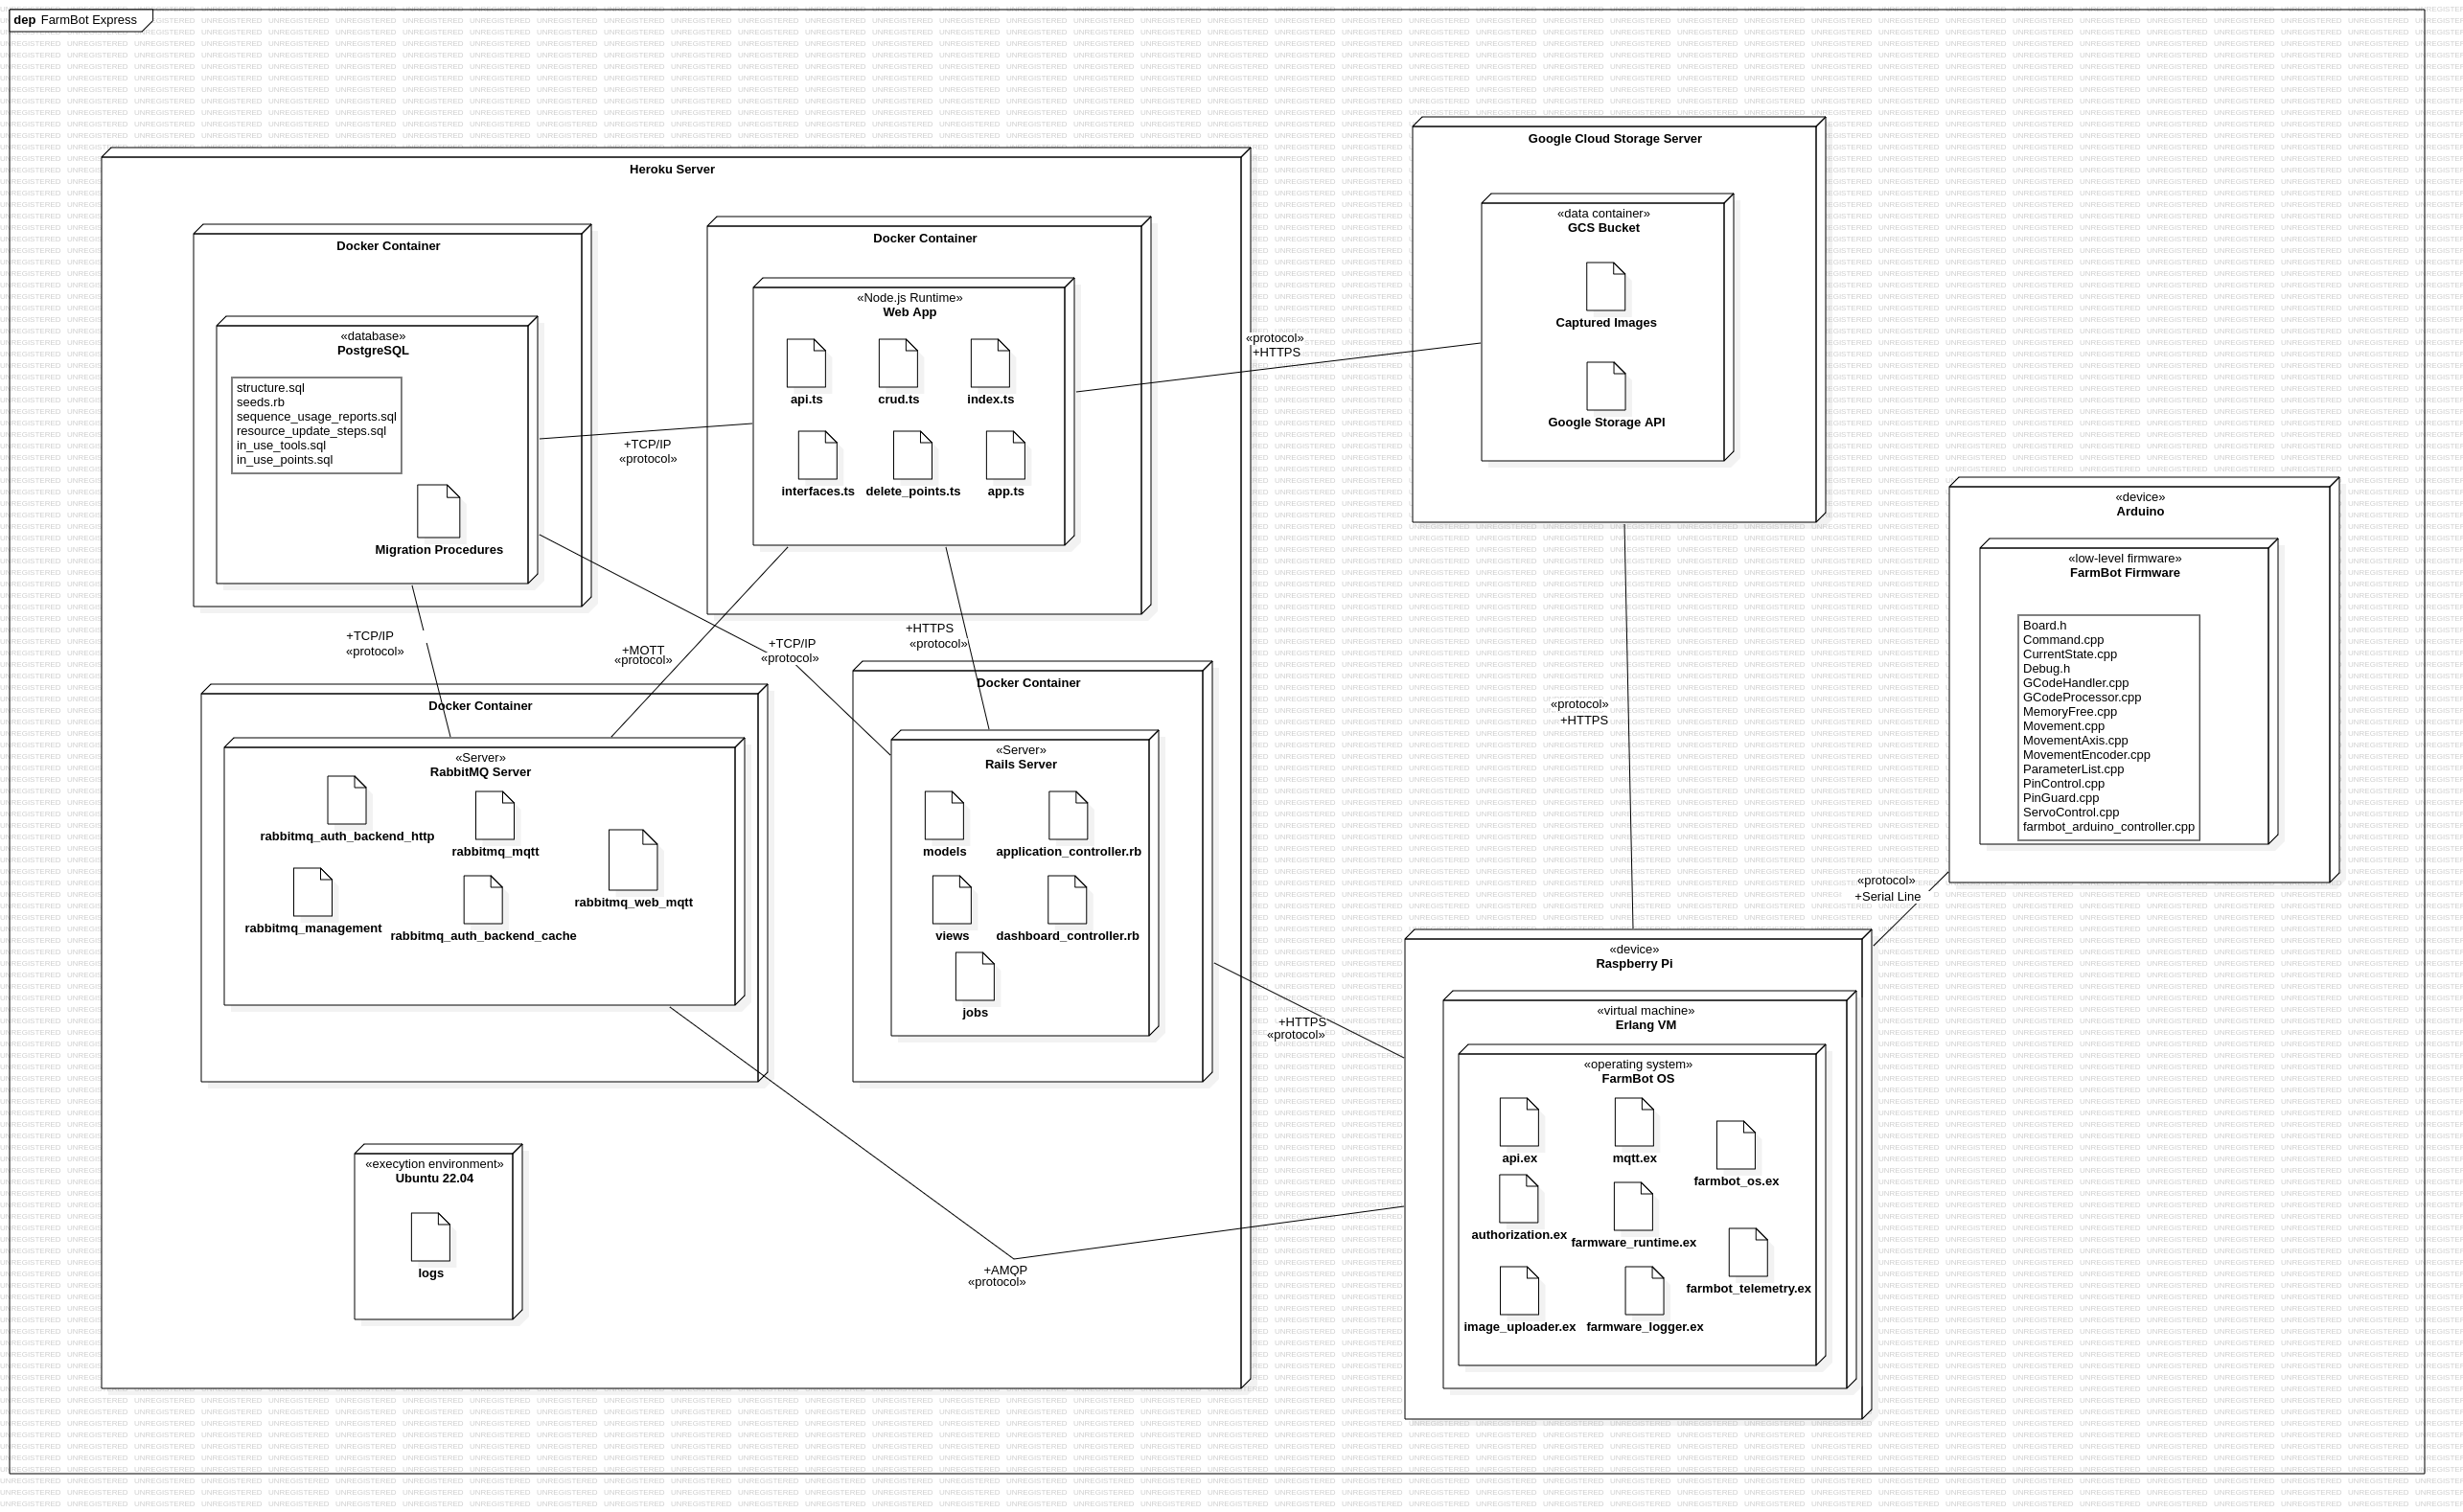
\includegraphics[width=1\textwidth]{Figures/DeploymentDiagram.png}
    \caption{FarmBot Deployment Diagram}\label{fig:DeploymentDiagram}
\end{figure}

The deployment diagram depicts the cloud-based FarmBot system architecture in which a central server manages updates, a Raspberry Pi controller runs the core application and a web application provides the user interface. The web application and the servers are deployed on Heroku. It's highly containerized. Docker containers are used for the PostgreSQL database, the Node.js runtime for the frontend, the RabbitMQ server used as the message broker, and Rails server used for backend. The containers run on a Ubuntu based machine. Besides the FarmBot Web App, Google Cloud Storage is used as an external datastore for storing images. FarmBot OS, an Elixir based operating system, is deployed on a Raspberry Pi Controller using Erlang VM. It communicates with the FarmBot firmware running on Arduino using low-level G and F codes. The firmware is responsible for controlling the hardware such as motors, sensors, actuators.
\section{Design Rationale}
% State \textbf{one rationale} specifically referring to each view presented

\begin{itemize}
    \item \textbf{Context View:}
          In the context of \textbf{FarmBot Express}, the Context View plays a particularly important role in elucidating how various external entities interact with the system. This view sheds light on how users engage with \textbf{FarmBot Express}, how developers contribute to its maintenance and updates, how the system fetches vital plant data from OpenFarm to inform agricultural decisions, and how it seamlessly integrates with GitHub for retrieving and incorporating the latest source code. This transparency empowers stakeholders to grasp the complete user experience, development workflow, data acquisition process, and software update mechanisms within the \textbf{FarmBot Express} ecosystem.
    \item \textbf{Functional View:} The Functional View, divides the system into three components. The Web app provides external interfaces to the end user to interact with, communicates with the FarmBot hardware through internal interfaces. FarmBot OS and Arduino firmware control hardware actions. The maintainability of the system is achieved with this separation of concerns.
    \item \textbf{Information View:} The Information View plays a critical role in deciphering FarmBot Express's data landscape. This view delves into the system's data requirements, outlining how data is stored, managed, and processed. Stakeholders gain valuable insights into the system's data model, allowing them to comprehend the structure and organization of information. Additionally, the Information View clarifies data flow throughout the system, providing transparency into how data is exchanged, manipulated, and utilized within FarmBot Express. This understanding empowers stakeholders to make informed decisions regarding data management strategies and ensures the system effectively handles the information crucial for its operation.
    \item \textbf{Deployment View:} The deployment conforms with the methodology of 12 Factor App. This ensures that the application is suitable to be deployed on modern cloud platforms, enables continuous deployment, can scale-up and offers maximum portability. 
    For particular decision rationales: \begin{itemize}
        \item Google Cloud Storage is used because uploading large files such as image files can take longer than 30 seconds on slow internet connections and for web applications that block requests, it can result in timout. Therefore, Heroku suggests directly uploading to a data bucket.
        \item A message broker is used because some interactions do not work well with the request/response pattern. We do not want to constantly check the API for messages. Instead, messages shall be received as soon as they are created without explicitly asking for them. Also, message brokers offer remote procedure calls and real-time data syncing.
    \end{itemize} 
\end{itemize}